\chapter{Interface}

\section*{Implémentation des layouts}
\paragraph{}
Les layouts sont la mise en forme des différentes pages de l'application. Android propose des attributs prédéfinis pour paramétrer l'affichage des composants (chaque composant Android est une View). Nous avons été plus loin que les attributs prédéfinis en Android : Christophe souhaitait par exemple avoir des éléments avec des bords arrondis, des background en couleur dégradées, etc.
Pour cela, il a fallu utiliser les drawable, a définir dans une fichier Xml, puis a appliquer sur les View concernées : 

\begin{center}
	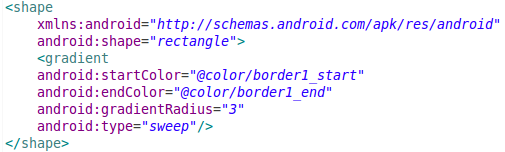
\includegraphics[width=140mm]{images/drawable.png}
	Drawable définissant les bords arrondis
\end{center}

\paragraph{}
Les différentes listes visibles dans l'application (par exemple la liste des fonctionnalités sur le menu principal) sont gérées par un fichier Xml qui défini la liste en elle même, et un fichier Xml qui définit un élément de cette liste. La encore il s'agit d'étendre ce qui est offert de base par android : les items d'une listview par défaut ne peuvent contenir qu'une String, alors que dans notre cas nous voulons afficher une icone et une String. Cela est rendu possible par l'heritage de la classe Adapter. Dans le cas d'une listview que l'on veut mettre a jour au cours de la vie de l'application, il faut implémenter la méthode notifyDataSetChanged() et l'appeler explicitement afin de rafraichir la ListView.

\begin{center}
	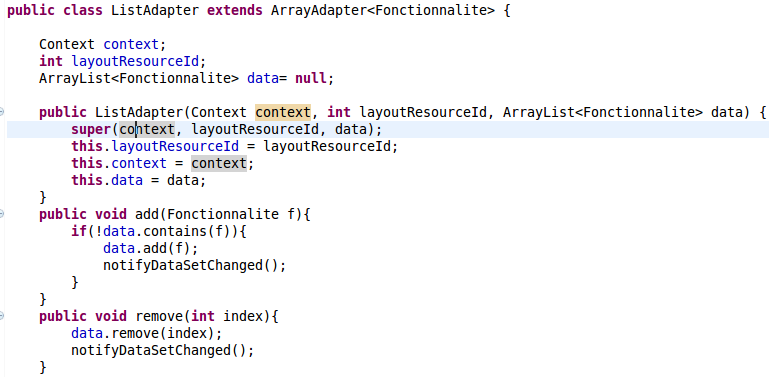
\includegraphics[width=140mm]{images/list_adapter.png}
	Adapter permettant la création d'un listview personnalisée
\end{center}

\paragraph{}
Lorsque nous avons testé l'application sur une tablette, nous nous sommes apercus que l'affichage du menu était trop petit sur une tablette, et lorsqu'il était correct sur tablette, les éléments étaient trop grand sur telephone. Nous avons gérer ces deux cas en détectant le périphérique sur lequel est lancé l'application et en appliquant un layout différent.

\begin{center}
	\fbox{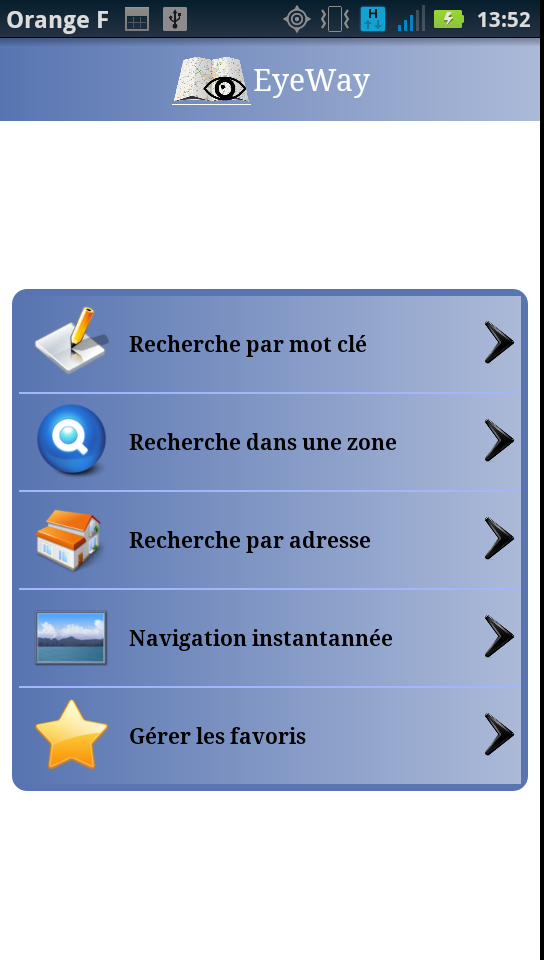
\includegraphics[width=60mm]{images/menu_principal.png}}
\end{center}

\begin{center}
	\fbox{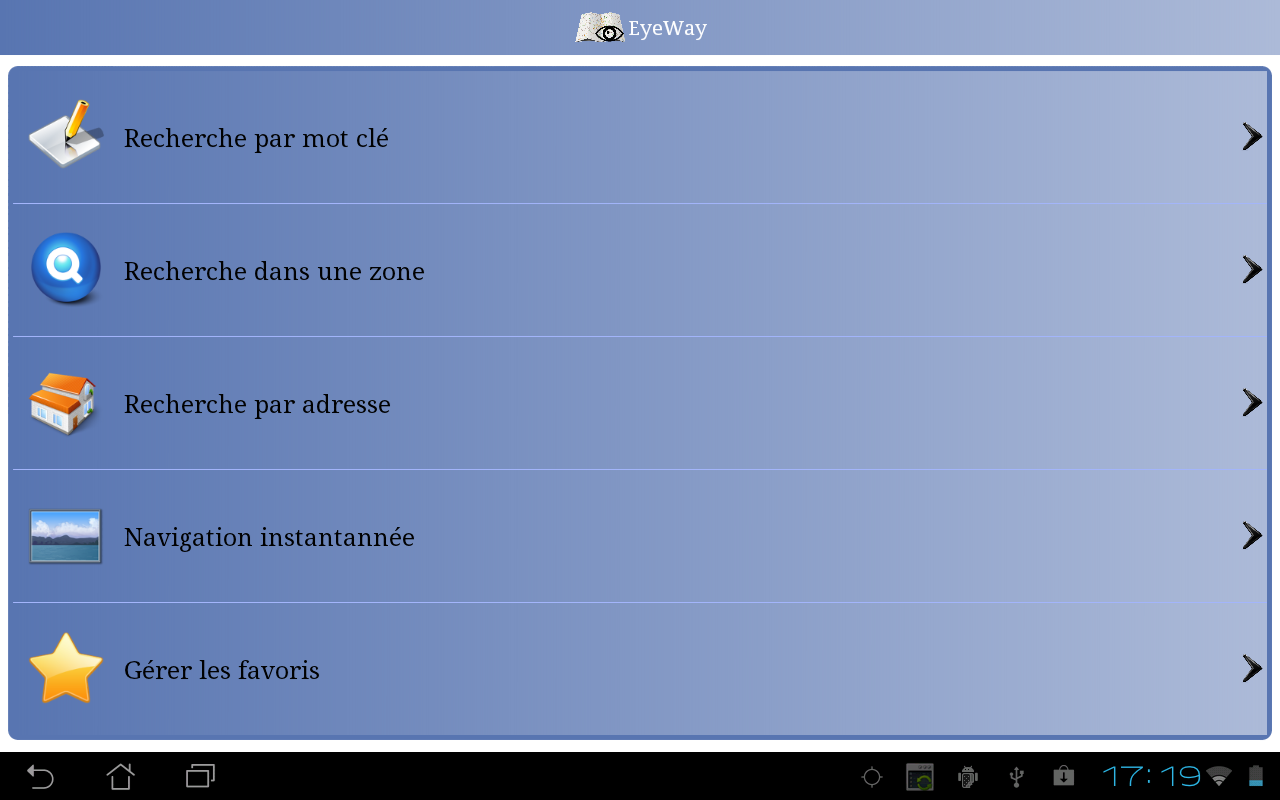
\includegraphics[width=140mm]{images/menu_tablette.png}}
\end{center}

\paragraph{}
Nous avons créer un bandeau contenant le nom et l'icône de l'application visible sur chaque page. Ce bandeau consiste en un fichier xml, chargé par les différents layout grâce à la directive include.
\section*{Gestion du swipe}
\paragraph{}
Nous avons implémenté le swipe sur différents formulaires afin de revenir sur le menu principal.

\section*{Gestion de l'orientation}
\paragraph{}
Lorsque l'orientation du terminal change, android fait un appel au onCreate() de l'application, ce qui a pour effet de perdre les saisies de l'utilisateur. C'est le cas dans la recherche par perimètre avec la liste des types extensible.
Nous avons géré le changement d'orientation en restaurant les types saisis par le passé.

\section*{AlertDialog customisée}
\paragraph{}
De base, Android ne permet de créer que des AlertDialog contenant un texte, et pour afficher un favoris ou bien un résultat de la recherche, nous avions besoin d'afficher le nom du lieu, l'adresse, la ville, le site web...
Nous avons utilisé des AlertDialog customisés, qui contiennent un layout définit la encore par un fichier Xml. 

\begin{center}
	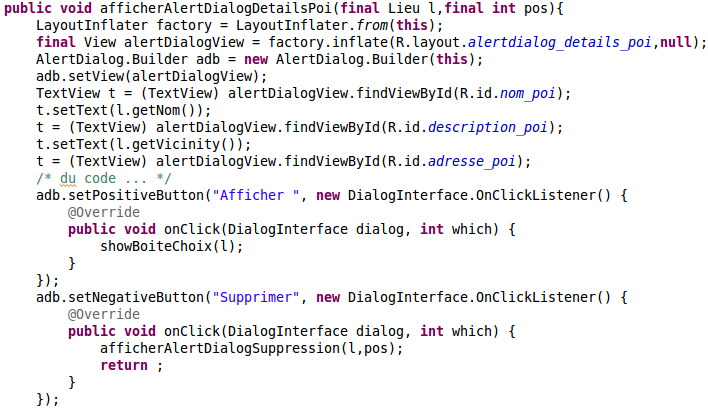
\includegraphics[width=140mm]{images/alertdialog.png}
	AlertDialog permettant de voir un favoris enregistré 
\end{center}
\paragraph{}
On a aussi construit une classe AlertDialogManager qui permet de contenir la définition des AlertDialog personnalisés de l'application, de manière a factoriser le code et a le rendre simple a utiliser.

\section*{Choix de l'affichage}
Pour chaque formulaire il est possible de consulter les résultats via la map ou la réalité augmentée par le biais d'une boite de dialogue.

\begin{center}
	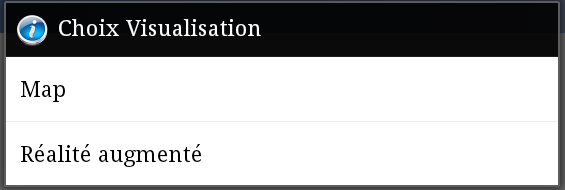
\includegraphics[width=140mm]{images/choix.png}
\end{center}


\section*{Affichage et sauvegarde des favoris}

\paragraph{}
Nous avons géré la sauvegarde d'un point d'intéret, de manière a ce que l'utilisateur puisse conserver les lieux qu'il a consulté. Pour cela, l'utilisateur peut rester appuyé sur l'ecran de réalité augmentée ou bien lorsqu'il consulte le détail d'un résultat.
\paragraph{}
L'affichage est confié a une listview extensible et rafraichie automatiquement (comme expliqué précédemment pour la listview des types pour la recherche par perimètre). 
\paragraph{}
La sauvegarde des favoris est faite avec des enregistrements dans l'internal storage Android.
Pour enregistrer un Lieu, il faut que cette classe soit serializable, puis il faut convertir l'objet concerné en tableau de bytes, et appeler la méthode write() :

\begin{center}
	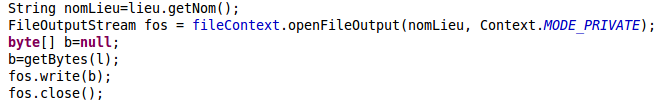
\includegraphics[width=140mm]{images/fichier.png}
\end{center}


\paragraph{}
Nous conservons dans l'application les favoris enregistrés, et il est possible de supprimer un favoris, ce qui va supprimer le fichier concerné dans l'internal storage.
